\documentclass[onecolumn, draftclsnofoot,10pt, compsoc]{IEEEtran}
\usepackage{graphicx}
\usepackage{url}
\usepackage{setspace}
\usepackage{float}
\usepackage{geometry}
\geometry{textheight=9.5in, textwidth=7in}

% 1. Fill in these details
\def \CapstoneTeamName{			Velocity-Raptors}
\def \CapstoneTeamNumber{		37}
\def \GroupMemberOne{			Alex Bailey}
\def \GroupMemberTwo{			Dylan Washburne}
\def \GroupMemberThree{			Benjamin Wick}
\def \CapstoneProjectName{		Object Velocity Tracking}
\def \CapstoneSponsorCompany{}
\def \CapstoneSponsorPerson{		Alex Neighbors}

% 2. Uncomment the appropriate line below so that the document type works
\def \DocType{		%Problem Statement
				Requirements Document
				%Technology Review
				%Design Document
				%Winter Progress Report
				}
			
\newcommand{\NameSigPair}[1]{\par
\makebox[2.75in][r]{#1} \hfil 	\makebox[3.25in]{\makebox[2.25in]{\hrulefill} \hfill		\makebox[.75in]{\hrulefill}}
\par\vspace{-12pt} \textit{\tiny\noindent
\makebox[2.75in]{} \hfil		\makebox[3.25in]{\makebox[2.25in][r]{Signature} \hfill	\makebox[.75in][r]{Date}}}}
% 3. If the document is not to be signed, uncomment the RENEWcommand below
%\renewcommand{\NameSigPair}[1]{#1}

%%%%%%%%%%%%%%%%%%%%%%%%%%%%%%%%%%%%%%%
\begin{document}
\begin{titlepage}
    \pagenumbering{gobble}
    \begin{singlespace}
    	
\includegraphics[height=4cm]{coe_v_spot1}
        \hfill 
        % 4. If you have a logo, use this includegraphics command to put it on the coversheet.
        %\includegraphics[height=4cm]{CompanyLogo}   
        \par\vspace{.2in}
        \centering
        \scshape{
            \huge CS Capstone \DocType \par
            {\large\today}\par
            \vspace{.5in}
            \textbf{\Huge\CapstoneProjectName}\par
            \vfill
            {\large Prepared for}\par
            \Huge \CapstoneSponsorCompany\par
            \vspace{5pt}
            {\Large\NameSigPair{\CapstoneSponsorPerson}\par}
            {\large Prepared by }\par
            Group\CapstoneTeamNumber\par
            % 5. comment out the line below this one if you do not wish to name your team
            %\CapstoneTeamName\par 
            \vspace{5pt}
            {\Large
                \NameSigPair{\GroupMemberOne}\par
                \NameSigPair{\GroupMemberTwo}\par
                \NameSigPair{\GroupMemberThree}\par
            }
            \vspace{20pt}
        }
        \begin{abstract}
        % 6. Fill in your abstract    
%Using a stationary camera, with the intent of being mounted on a car, we are attempting to  detect objects and determine the velocities of those objects relative to the Observer (camera).
Using a stationary camera, we are attempting to detect objects and determine the velocities of those objects relative to the Observer (camera).
This will be done by having the camera recognize a specific type of object, either people or RC cars, in space and determine their velocities based on the rate at which they travel through the frame.
The speed of the objects will be displayed in a windows application.
This project is intended to be a proof of theory.         
        \end{abstract}     
    \end{singlespace}
\end{titlepage}
\newpage
\pagenumbering{arabic}
\tableofcontents
% 7. uncomment this (if applicable). Consider adding a page break.
%\listoffigures
%\listoftables
\clearpage

% 8. now you write!

%Beginning of introduction
\section{Introduction}
\subsection{Purpose}
The purpose of this document is to present a detailed description of the requirements for the "Video Radar" software.
This document is intended for the main use of the client, as well as the professor and the teacher assistants and will be proposed to the client for its approval.

\subsection{Scope}
Our product, the "Video Radar", will be able to identify a specific type of object, such as a person or an RC car, calculate the object's velocity, then display the speed onto a windows application.
Our project is intended to be proof of concept in which it may be implemented in many different ways by others.
We intend to limit our objects to either people or RC cars, while in theory the system may track any object the user wants.
This system must be used indoors because the Kinect uses infrared sensors that will not function correctly outside.
\subsection{Definitions, Acronyms, and Abbreviations}
\begin{tabular}{|p{4cm}|p{12cm}|}
	\hline
	\textbf{Term} & \textbf{Definition} \\
	\hline
	API (Application Program Interface) & A particular set of rules and specifications that software programs can follow to communicate with each other. \\
	\hline
    Computer Vision & Tasks that involve analyzing a video feed to produce symbolic information.  \\
	\hline
	Object & The entity being tracked by the video feed.  \\
	\hline
    Speed & The rate at which an object covers distance.  \\
	\hline
    Velocity & The rate at which an object changes its position.  \\
	\hline
	
\end{tabular}



\subsection{Overview}
The rest of the document contains two additional sections.
The first section is the overall description.
This section will describe the intended use of the software and give background.
The last section is the specific requirements section.
This section contains all the software requirements.

%Beginning of overall description
\section{Overall Description}
\subsection{Product Perspective}
Our product will be a self-contained product. 
Our product's interface will consist of a window where the user can activate the camera and velocity tracking.
There will be a menu bar in the application that will allow the user to specify aspects of the product, as shown by Section C in the picture A below.
There will be a table on the side of the application, Section D of picture A, that will have a list objects being tracked and their speed.
Our products application window will consist of a small button row at the bottom for essential buttons, such as the start and stop buttons, as depicted in Section B of picture A below.
The application will have a central section for displaying the video captured by the camera with our information overlay, such as Section A of picture A below.
We will be using computer vision software in order to identify the type of object and track its location across the frame.
The product will have only one mode of operation, the on mode, where the product constantly processes the images from the camera and velocity is displayed.
This mode requires no input from the user except to turn off.
The camera will not have any automated motion.
The user will have to manually adjust the camera.
The camera will have a fixed zoom that the user will not be able to change.

\begin{figure}[ht]
    \centering
    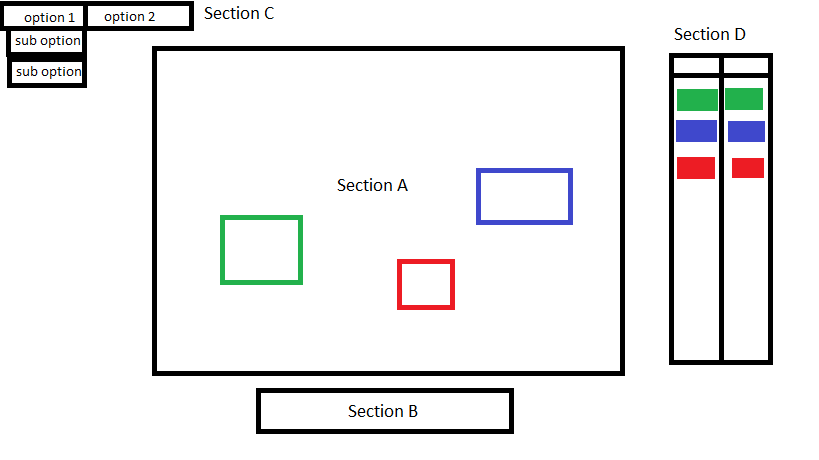
\includegraphics[scale=0.75]{cs_461_mock_up}
    \caption{Picture A: Mock-Up of the Application Window}
    \label{fig: pic_a}
\end{figure}


\subsection{Product Functions}
The software will be connected to a camera with a live video feed.
It will then be able to detect objects that are specified for the users needs.
The software will then be able to acquire the velocity at which the objects are traveling.
%This information will be stored into a table for the user to see.


%REWRITE 
\subsection{User Characteristics}
%This software is intended to be used by many different users.
% The types of users are broken down into two categories: users who wish to track cars, users who wish to track people.
% These users have different use for the product but the software should work the same way for both users.

% Users who wish to track cars may use the product to detect the velocity of a moving car on the road.
% This means the user will set the stationary camera and point it in the direction of moving vehicles to obtain the velocity.

% Users who wish to track the velocity of people may also use the product.
% These users will follow the same procedure as the other users but instead, the software will detect the velocity of people.

This software is intended to be used by many different users. 
Because we have yet to decide on the specific type of object to track, the education level and experience is not for certain. 
However, because our product is meant to replace current methods of object velocity tracking, such as the radar gun, our intended users will not need a high education or experience level. 
In fact it will probably be expected that minimal training is needed to operate our product.

In order to examine the possible users for our product, we will examine possible object types.

If we decide to use cars as our object type, the main users would be police officers, to be used in enforcing speed limits. 
In this case the user would have good education level, but likely not high technical expertise.

If we decide to use people as our object type, then the main users will likely be analysists, analyzing human movement patterns and speeds in various contexts such as sports or emergency evacuation. In this case, our users will be highly educated, but they too would likely not have high technical expertise.

\subsection{Constraints}
This product will likely require a nontrivial amount of resources to perform its task at the constant interval we require.
As a result, our product will either need to come with a dedicated computer to do the processing, or it will have to interface with existing computers which we expect to be in the locations of use.

In accordance with federal laws, the camera is allowed to be recording anything described as "within plain sight".
The proper use of this falls on the user, and must be disclaimed before use.

The product's reliability of use can be described in a number of ways.
The camera should be recording at a constant and stable rate.
The objects in the scene should be properly identified with 70\% accuracy.
The tracking of an identified object's velocity should be within 90\% of the objects actual velocity.
%The velocity tracking should also be reliably given every 0.5 seconds, without any notable dips in rate of recording and processing.
The velocity tracking should also be reliably given every 0.5 seconds, with 30 frames per second 90\% of the time.

While the video recorded is protected by federal laws, the information nonetheless must meet certain security standards.
If the video data is to be saved locally, it should also respect encryption of the product it is saved on.
%Should the video be live streamed to a remote location, it must enter a stable connection to deliver to the intended viewer.

\subsection{Assumptions and Dependencies}
We assume that if our products camera needs to move that our product would be able to either handle the motion of the camera and still be able to track velocities or be mounted securely enough to minimize motion of the camera, allowing the product to track velocities.
We assume that the computer vision software will be able to recognize an object within enough time after entering the frame so that there will be enough time for the velocity algorithm to calculate the velocity.

%Beginning of specific requirments
\section{Specific Requirements}
%I don't know about the "cross-reference" part, I'm just ignoring that for now
The product must be able to identify objects in frame, and differentiate them from the background.
%The product must identify desired objects at least 70\% of the time while they are in frame.
When the product identifies an object as the desired type, at least 70\% of the time this must actually be the desired object type.

The product must be able to track the velocities of identified objects.
For each object identified in the scene, the velocity the program displays to the user must be within 90\% of the objects true velocity.

The product must have the capability to identify and track multiple objects simultaneously.
%It must be able to track as many objects as it can identify, however we would like the product to be able to identify up to 6 objects at once under most setup conditions. 
It must be able to identify and track at least 4 objects simultaneously.
At the same time, should the proper conditions present themselves, the product should be able to automatically identify as many objects it can locate in frame, should that number exceed 4.

%Parallel and perpendicular
The product should be able to perform its velocity analysis on objects that are moving in various directions.
While it should track the velocities of objects moving perpendicular to the camera, it should also be able to identify the velocities of objects moving parallel to the camera, or at any variation in between.
The velocities returned are within 90\% of the objects' true speeds, as stated above, however direction should not cause the product to fail its purpose.

%Max effective view distance of 100m
The product will accurately work within 10m of the camera's placement.
Objects within 10m of the camera's placement, within its view angle and with an unobstructed line of sight, should all be able to be identified by the camera, adhering to the accuracy requirements described above.
Objects beyond the maximum effective range can potentially still be identified if the conditions allow, but are not granted the same accuracy guarantee.
%User interface
Our product's interface will consist of a window where the user can activate the camera and velocity tracking as well as view the camera input live, with squares surrounding each object being tracked and speeds posted below the squares.
There will be a menu bar in the application that will allow the user to specify aspects of the product, as shown by Section C in the picture A above.
There will be a table on the side of the application, Section D of picture A, that will have a list objects being tracked and their speed.
These values will be saved to a comma separated value text document for later analysis.
Our products application window will consist of a small button row at the bottom for essential buttons, such as the start and stop buttons, as depicted in Section B of picture A above.
The application will have a central section for displaying the video captured by the camera with our information overlay, such as Section A of picture A above.

\newpage

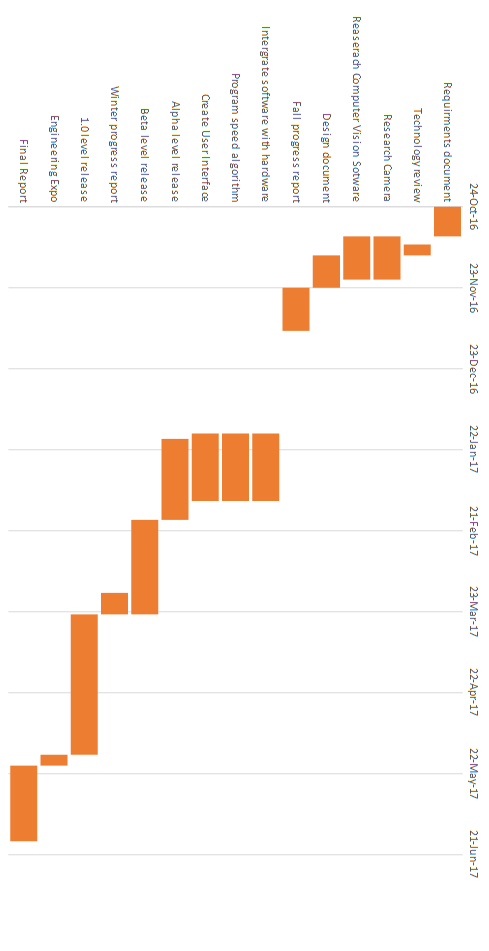
\includegraphics[scale=1]{gantt}

\end{document}